\documentclass{article}
\usepackage[UTF8]{ctex}
\usepackage[utf8]{inputenc} % allow utf-8 input
\usepackage[T1]{fontenc}    % use 8-bit T1 fonts
\usepackage{hyperref}       % hyperlinks
\usepackage{url}            % simple URL typesetting
\usepackage{booktabs}       % professional-quality tables
\usepackage{amsfonts}       % blackboard math symbols
\usepackage{nicefrac}       % compact symbols for 1/2, etc.
\usepackage{microtype}      % microtypography
\usepackage{lipsum}
\usepackage{geometry}
\usepackage{graphicx} %插入图片的宏包
\usepackage{float} %设置图片浮动位置的宏包
\usepackage{subfigure} %插入多图时用子图显示的宏包
\usepackage{listings}
\usepackage{amsthm}
\usepackage{tikz}

\theoremstyle{definition}
\newtheorem{theorem}{\indent 定理}[section]
\newtheorem{lemma}[theorem]{\indent 引理}
\newtheorem{proposition}[theorem]{\indent 命题}
\newtheorem{corollary}[theorem]{\indent 推论}
\newtheorem{definition}{\indent 定义}
\newtheorem{example}{\indent 例}
\newtheorem{remark}{\indent 注}
\newenvironment{solution}{\begin{proof}[\indent\bf 解]}{\end{proof}}
\renewcommand{\proofname}{\indent\bf 证明}

\usepackage[utf8]{inputenc}
\usepackage[T1]{fontenc}
\usepackage{pgfplots}
\usetikzlibrary{calc}
\pgfplotsset{compat=1.12}
    
\pgfplotsset{
    compat=1.12,
}

\geometry{a4paper,scale=0.8}
\date{}

\usepackage{listings}
\usepackage{color}

\definecolor{dkgreen}{rgb}{0,0.6,0}
\definecolor{gray}{rgb}{0.5,0.5,0.5}
\definecolor{mauve}{rgb}{0.58,0,0.82}

\lstset{frame=tb,
  language=Python,
  aboveskip=3mm,
  belowskip=3mm,
  showstringspaces=false,
  columns=flexible,
  basicstyle={\small\ttfamily},
  numbers=none,
  numberstyle=\tiny\color{gray},
  keywordstyle=\color{blue},
  commentstyle=\color{dkgreen},
  stringstyle=\color{mauve},
  breaklines=true,
  breakatwhitespace=true,
  tabsize=3
}

\title{椭圆曲线密码}


\author{
Elliptic Curve Cryptography\\
 刘卓\\
 \texttt{ } \\
}


\begin{document}
\maketitle

由Miller和Koblitz在20世纪80年代中期提出。大约在同一时间,Lenstra开发了一种使用椭圆曲线的分解算法。近年来,椭圆曲线在密码学中的应用得到了迅速的发展。其主要优点是利用椭圆曲线,我们可以用比RSA和其他现代密码系统所需要的数目小得多的数字来实现安全性。

\section{椭圆曲线}

\begin{definition}[椭圆曲线] 
实数上的椭圆曲线是满足方程的点$(x, y)$的集合
$$E:y^2 = x^3+Ax+B, A,B \in \mathbb{R}$$
要求曲线是非奇异(non-singular)的(即无尖端、无自交、无孤立点)。这个条件等价于
$$4A^3 + 27 B^2  \ne 0$$
\end{definition}

\begin{example}

椭圆曲线$y^2=x^3-3x+3$:

~\\
$$
\begin{tikzpicture}
    \begin{axis}[
        xmin=-3,
        xmax=6,
        ymin=-5,
        ymax=5,
        xlabel={$x$},
        ylabel={$y$},
        scale only axis,
        axis lines=middle,
        % set the minimum value to the minimum x value
        % which in this case is $-\sqrt[3]{7}$
        domain=-2.1038:3,%需要求根
        samples=1000,
        smooth,
        % to avoid that the "plot node" is clipped (partially)
        clip=false,
        % use same unit vectors on the axis
        axis equal image=false,
    ]
        \addplot [red] {sqrt(x^3-3*x+3)}
            node[right] {$y^2=x^3-3x+3$};
        \addplot [red] {-sqrt(x^3-3*x+3)};
    \end{axis}
\end{tikzpicture}
$$
$$4A^3 + 27 B^2  = 4 \cdot (-3)^3 + 27 \cdot 3^2 \ne 0$$


\end{example}
$\hfill\square$ 

点$P = (x_P,y_P)$和点$Q = (x_Q,y_Q)$是在椭圆曲线$E:y^2 = x^3+Ax+B$上的两个点。则$P+Q = (x_R,-y_R)$,其中

\begin{eqnarray}   
\label{eq}
\alpha &=&\frac{y_{Q}-y_{P}}{x_{Q}-x_{P}}\nonumber \\ 
x_{R}&=&\alpha^{2}-x_{P}-x_{Q} \nonumber \\ 
y_{R} &=&y_{P}+\alpha\left(x_{R}-x_{P}\right)\nonumber \\ 
\nonumber 
\end{eqnarray}

\begin{example}

$$
    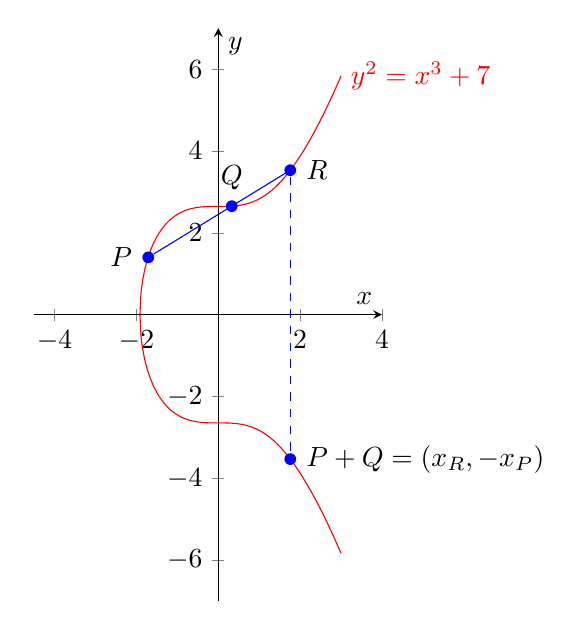
\begin{tikzpicture}[
        % define the style `point' which is used for the nodes on the coordinates
        point/.style={
            circle,
            fill=blue,
            inner sep=1.5pt,
        },
    ]
        \begin{axis}[
            xmin=-4.5,
            xmax=4,
            ymin=-7,
            ymax=7,
            xlabel={$x$},
            ylabel={$y$},
            scale only axis,
            axis lines=middle,
            % set the minimum value to the minimum x value
            % which in this case is $-\sqrt[3]{7}$
            domain=-1.912931:3,
            samples=200,
            smooth,
            % to avoid that the "plot node" is clipped (partially)
            clip=false,
            % use same unit vectors on the axis
            axis equal image=true,
        ]
            \addplot [red] {sqrt(x^3+7)}
                node[right] {$y^2=x^3+7$};
            \addplot [red] {-sqrt(x^3+7)};

            % add nodes to the points and the corresponding labels
            \node [point,label={left:$P$}]
                (P) at (-1.71,1.4)  {};
            \node [point,label={above:$Q$}]
                (Q) at (0.33,2.65)  {};
            \node [point,label={right:$R$}]
                (R) at (1.76,3.53)  {};
            \node [point,label={right:$P + Q = (x_{R},-x_{P}) $}]
                (PQ) at (1.76,-3.53)  {};

            % draw a line from (P0) a bit further than just to (P3)
            \draw [blue] (P) -- ($ (P)!1!(R) $);
            \draw [blue,dashed] (R) -- ($ (R)!1!(PQ) $);
        \end{axis}
    \end{tikzpicture}
$$

\end{example}
$\hfill\square$ 

\begin{definition}如果点$P = (x_P,y_P)$在椭圆曲线$E:y^2 = x^3+Ax+B$上,$2P = (x_R,-y_R)$,其中

\begin{eqnarray}   
\label{eq}
\alpha &=&\frac{3x_P^2+A}{2y_P}\nonumber \\ 
x_{R}&=&\alpha^{2}-2x_{P} \nonumber \\ 
y_{R} &=&y_{P}+\alpha\left(x_{R}-x_{P}\right)\nonumber \\ 
\nonumber 
\end{eqnarray}
\end{definition}

\begin{example}

$y^2 = x^3+3x+5; P = (-1,1), \mbox{计算}2P$

\begin{eqnarray}   
\label{eq}
\alpha &=&\frac{3x_P^2+A}{2y_P} = \frac{3(-1)^2+3}{2(1)} = 3\nonumber \\ 
x_{R}&=&\alpha^{2}-2x_{P} = 3^2 - 2(-1)= 11 \nonumber \\ 
y_{R} &=&y_{P}+\alpha\left(x_{R}-x_{P}\right) = 1 + 3(11- (-1)) = 37\nonumber \\ 
2P &=&\left(x_{R}-y_{R}\right) = (11,-37)
\nonumber 
\end{eqnarray}

$$
    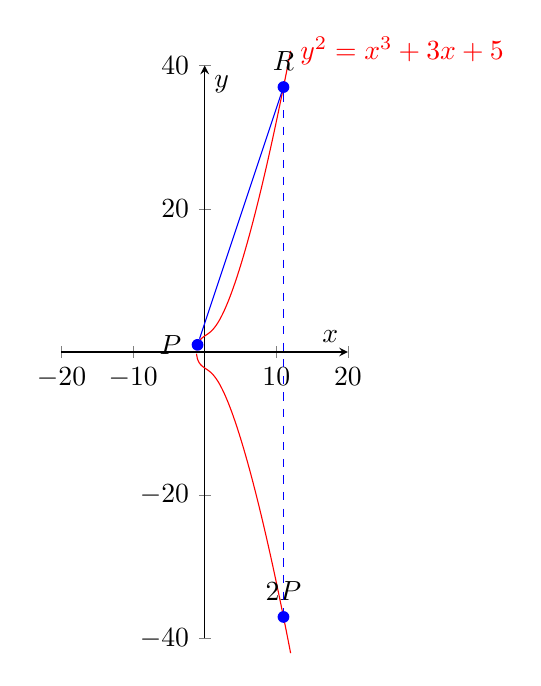
\begin{tikzpicture}[
        % define the style `point' which is used for the nodes on the coordinates
        point/.style={
            circle,
            fill=blue,
            inner sep=1.5pt,
        },
    ]
        \begin{axis}[
            xmin=-20,
            xmax=20,
            ymin=-40,
            ymax=40,
            xlabel={$x$},
            ylabel={$y$},
            scale only axis,
            axis lines=middle,
            % set the minimum value to the minimum x value
            % which in this case is $-\sqrt[3]{7}$
            domain=-12:12,
            samples=200,
            smooth,
            % to avoid that the "plot node" is clipped (partially)
            clip=false,
            % use same unit vectors on the axis
            axis equal image=true,
        ]
            \addplot [red] {sqrt(x^3+3*x+5)}
                node[right] {$y^2 = x^3+3x+5$};
            \addplot [red] {-sqrt(x^3+3*x+5)};

            % add nodes to the points and the corresponding labels
            \node [point,label={left:$P$}]
                (P) at (-1,1)  {};
            \node [point,label={above:$2P$}]
                (2P) at (11,-37)  {};
            \node [point,label={above:$R$}]
                (R) at (11,37)  {};


            % draw a line from (P0) a bit further than just to (P3)
            \draw [blue] (P) -- ($ (P)!1!(R) $);
            \draw [blue,dashed] (R) -- ($ (R)!1!(2P) $);
        \end{axis}
    \end{tikzpicture}
$$
\end{example}
$\hfill\square$ 


\begin{definition}
给定一个质数$p$,一个(离散的)椭圆曲线并mod $p$是满足方程的所有整数点(x, y)的集合,该方程表示为:
$$E:y^2 = x^3+Ax+B \pmod{p}$$
$$A,B \in [0, p-1],4A^3+27B^2 \ne 0 \pmod{p} $$

\end{definition}

\begin{example}

$y^2 = x^3+16x+14 \pmod{23}$

$$
\left(\begin{array}{c|cccccccccccccccccccccc}
x & 1 & 2 & 3 & 4 & 5 & 6 & 7 & 8 & 9 & 10 & 11 & 12 & 13 & 14 & 15 & 16 & 17 & 18 & 19 & 20 & 21 & 22 \\
y^2 \pmod{23}& 8 & 8 & 20 & 4 & 12 & 4 & 9 & 10 & 13 & 1 & 3 & 2 & 4 & 15 & 18 & 19 & 1 & 16 & 1 & 8 & 20 & 20
\end{array}\right)
$$

比如$\underbrace{y^2 = 10^2 = ${\color{red}8}$  = 1^3+16 \cdot 1 +14 = x^3+16x+14}_{\pmod{23}}$,所以$(1,10)$为一个解

再者$\underbrace{y^2 = 13^2 = ${\color{red}8}$  = 2^3+16 \cdot 2 +14 = x^3+16x+14}_{\pmod{23}}$,所以$(2,13)$为一个解

所有32个解的集合为
$$
\begin{array}{l}
\{\{1,10\},\{1,13\},\{2,10\},\{2,13\},\{4,2\},\{4,21\},\{5,9\}, \\
\{5,14\},\{6,2\},\{6,21\},\{7,3\},\{7,20\},\{9,6\},\{9,17\}, \\
\{10,1\},\{10,22\},\{11,7\},\{11,16\},\{12,5\},\{12,18\}, \\
\{13,2\},\{13,21\},\{15,8\},\{15,15\},\{17,1\},\{17,22\}, \\
\{18,4\},\{18,19\},\{19,1\},\{19,22\},\{20,10\},\{20,13\}\}
\end{array}
$$

\begin{lstlisting}
def Elliptic_Curve_points(A,B,p):
    """
    求解满足椭圆曲线y^2 = x^3 + Ax + B
    所以整数点的几何
    但对于大质数运算时间过长

    p : int
        质数,求余.
    A : int
        椭圆曲线A.
    B : int
        椭圆曲线B.

    返回所有点

    """
    return [(x, y) for x in range(p) for y in range(p) if (y*y - (x**3 + A*x + B)) % p == 0]

print(Elliptic_Curve_points( A=16, B=14, p=23))

\end{lstlisting}

\end{example}
$\hfill\square$ 


以下算式都适用于实数上的椭圆曲线和mod p的椭圆曲线:
\begin{itemize}
\item 加法结合律:$(P_1+P_2)+P_3 = P_1+(P_2+P_3)$;
\item 加法交换律:$P_1+P_2=P_2+P_1$;
\item 如果$P=(x,y)$并有一个整数$k$,则:
$$kP = \underbrace{P+P+ \cdots + P}_{\mbox{k个}}$$
\item 对于任意两个整数$k,h$,则
$$h(kP) = (hk)P =k(hP)$$
\end{itemize}

~\\

\begin{definition}[椭圆曲线加法]
让$P = (x_P,y_P)$和点$Q = (x_Q,y_Q)$是在椭圆曲线$E:y^2 = x^3+Ax+B \pmod{p}$上的两个点。则$P+Q = (x_R,-y_R)$,其中

\begin{eqnarray}   
\label{eq}
\alpha &=&\left(y_{Q}-y_{P}\right) \cdot\left(x_{Q}-x_{P}\right)^{-1} \pmod{p} \nonumber \\ 
x_{R} &=& \alpha^{2}-x_{P}-x_{Q}\pmod{p} \nonumber \\ 
y_{R} &=& y_{P}+\alpha\left(x_{R}-x_{P}\right) \pmod{p}\nonumber \\ 
\nonumber 
\end{eqnarray}
\end{definition}

\begin{definition}[椭圆曲线点倍增]
让$P = (x_P,y_P)$是在椭圆曲线$E:y^2 = x^3+Ax+B \pmod{p}$上的两个点。则$2P = (x_R,-y_R)$,其中

\begin{eqnarray}   
\label{eq}
\alpha &=&\left(3{x_P}^2 + A\right) \cdot\left(2y_P\right)^{-1} \pmod{p} \nonumber \\ 
x_{R} &=& \alpha^{2}-2x_{P}\pmod{p} \nonumber \\ 
y_{R} &=& y_{P}+\alpha\left(x_{R}-x_{P}\right) \pmod{p}\nonumber \\ 
\nonumber 
\end{eqnarray}
\end{definition}



\begin{example}
让$p = 23, y^2 = x^3+13x + 7 \pmod{23}$,点$P = (14,9)$,点$Q = (17,14)$
\begin{enumerate}
\item 点$P,Q$是否在曲线上?
~\\

\begin{solution}
$$A = 13;B = 7;p = 23$$
$$4A^3 +27B^2 \pmod{23} = 4 \cdot (13)^3 +27 \cdot (7)^2 \pmod{23} \ne 0$$
$$P = (14,9) \mbox{代入} y^2 = x^3+13x 7$$满足等式即可
\end{solution}
\item 计算$P+Q$
\begin{solution}
\begin{eqnarray}   
\label{eq}
\alpha &=&\left(y_{Q}-y_{P}\right) \cdot\left(x_{Q}-x_{P}\right)^{-1} \pmod{p}\nonumber \\ &=& (14-9)(17-14)^{-1}\pmod{23}\nonumber \\ 
&=& (5)(3)^{-1}\pmod{23}\nonumber \\ 
&=& (5)(8)\pmod{23}\nonumber \\ 
&=& 17 \pmod{23}\nonumber \\ 
&&\nonumber \\ 
x_{R} &=& \alpha^{2}-x_{P}-x_{Q}\pmod{p} \nonumber \\ 
&=& 17^2 - 17 - 14 \pmod{23}\nonumber \\ 
&=& 5 \pmod{23}\nonumber \\ 
&&\nonumber \\ 
y_{R} &=& y_{P}+\alpha\left(x_{R}-x_{P}\right) \pmod{p}\nonumber \\ 
&=& 9 + 17(5-14)\pmod{23}\nonumber \\ 
&=& 17\pmod{23}\nonumber \\ 
-y_{R}&=& -17\pmod{23}\nonumber \\ 
&=& 6\pmod{23}\nonumber \\ 
\nonumber 
\end{eqnarray}
$$P+Q = (x_{R},-y_{R})=(5,6)$$
\end{solution}
\item 如果$S = (9,5)$,$T = (9,18)$, 计算$S+T$
\begin{solution}
因为$y_T + y_S = 0 \pmod{23}$, 所以$S+T$无解
\end{solution}
\end{enumerate}
\end{example}

~\\

\begin{example}
让$p = 23, y^2 = x^3+5x + 8 \pmod{23}$,点$P = (3,2)$,计算$2P$

\begin{solution}
$A = 5;B = 8;p = 23$

\begin{eqnarray}   
\label{eq}
\alpha &=&\left(3{x_P}^2 + A\right) \cdot\left(2y_P\right)^{-1} \pmod{p} \nonumber \\ 
&=& (3(3)^2 + 5)\cdot (2(2))^{-1} \pmod{23} \nonumber \\ 
&=& (32)\cdot (4)^{-1} \pmod{23} \nonumber \\ 
&=& 9 \cdot 6\pmod{23} \nonumber \\ 
&=& 8 \pmod{23} \nonumber \\ 
&& \nonumber \\ 
x_{R} &=& \alpha^{2}-2x_{P}\pmod{p} \nonumber \\ 
&=& 64 - 2(3)\pmod{23} \nonumber \\ 
&=& 12\pmod{23} \nonumber \\ 
&& \nonumber \\ 
y_{R} &=& y_{P}+\alpha\left(x_{R}-x_{P}\right) \pmod{p}\nonumber \\ 
&=& 2 + 8(12-3)\pmod{23} \nonumber \\ 
&=& 5\pmod{23} \nonumber \\ 
- y_{R}&=& -5\pmod{23} \nonumber \\ 
&=& 18\pmod{23} \nonumber \\ 
\nonumber 
\end{eqnarray}
$$2P = (x_{R},-y_{R})=(12,18)$$
\end{solution}
\end{example}

\section{椭圆曲线迪菲-赫尔曼密钥交换}
\begin{enumerate}
\item ${\color{blue}Alice}$ 和 ${\color{red}Bob}$决定一个质数$p$,并在曲线$E_p:y^2 = x^3+Ax+B \pmod{p}$上选择一个点$Q$,并公开;
\item ${\color{blue}Alice}$随机选择一个整数$N_A$, ${\color{red}Bob}$随机选择一个整数$N_B$,并自己保留,不公开;
\item ${\color{blue}Alice}$ 计算$Q_A = N_A \cdot Q$ (这里$N_A \cdot Q$是指$N$倍的$Q$,方法与求$2P$相同)然后发送给 ${\color{red}Bob}$;
\item ${\color{red}Bob}$ 计算$Q_B = N_B \cdot Q$ 然后发送给 ${\color{blue}Alice}$;
\item ${\color{blue}Alice}$ 计算$N_B \cdot Q_A$;${\color{red}Bob}$ 计算$N_A \cdot Q_B$;
\item 因此他们得到公钥:
$$N_AQ_B=N_A(N_BQ)=(N_AN_B)Q=(N_BN_A)Q=N_B(N_AQ)=N_BQ_A$$
\end{enumerate}

~\\

其思想就是:

\begin{itemize}
\item 用曲线加法代替模乘$p$;
\item 用曲线上点的整数倍来代替模幂$p$;
\item 暂时没有已知算法可以分解攻击曲线密码;
\item 椭圆曲线的模可以用来分解$N$;
\item 离散对数的改版;
\end{itemize}

~\\

\begin{example}
${\color{blue}Alice}$ 和 ${\color{red}Bob}$ 想要交换一个密钥,因此他们共同决定了一个质数$p = 7211$ 和椭圆曲线$ E_{7211} : y^2 = x^3 +x+7206 \pmod{8831}$。并公开点$P = (3,5)$

\begin{enumerate}
\item ${\color{blue}Alice}$选择一个整数$N_A = 12$,然后计算$Q_A = N_A \cdot P = (1794,6375)$;
\item ${\color{red}Bob}$选择一个整数$N_B = 23$,然后计算$Q_B = N_B \cdot P = (3861,1242)$;
\item 保留$N_A,N_B$,公开$Q_A,Q_B$
\item ${\color{blue}Alice}$拿到了$Q_B$后计算$N_AQ_B = 12(1794,6375)  = (1472,2098)$
\item ${\color{red}Bob}$拿到了$Q_A$后计算$N_BQ_A= 23(3861,1242)  = (1472,2098)$
\end{enumerate}

因为$N_AQ_B=N_A(N_BQ)=(N_AN_B)Q=(N_BN_A)Q=N_B(N_AQ)=N_BQ_A$,因此他们成功交换了密钥。

\end{example}
$\hfill\square$ 

\subsection{发布明文}

现在${\color{blue}Alice}$ 和 ${\color{red}Bob}$决定一个质数$p$,并使用曲线$E_p:y^2 = x^3+Ax+B \pmod{p}$进行加密。

明文转化为整数$M \in [1,p-1]$

\begin{enumerate}
\item 选择一个大整数$k$,计算
$$x_j = M \cdot k, j \in {1,2,\cdots,k-1}$$
\item 每次计算$x_j$,我们测试$x^3+Ax+B$是否二次剩余mod $p$
\item 当第一次$x^3+Ax+B$二次剩余mod $p$,使用点$U$加密明文$M$,其中
$$U = \left(x_j,\sqrt{x_j^3+Ax_j+B}\right) \pmod{p}$$
\end{enumerate}


\section{椭圆曲线El Gamal}

\begin{enumerate}
\item ${\color{red}Bob}$决定一个质数$p$和一个椭圆曲线$E_p:y^2 = x^3+Ax+B \pmod{p}$。然后再选择一个点$P$和一个正整数$k$。计算$Q = k\cdot P$;
\item ${\color{red}Bob}$公开$E_p,P,Q$。保留$k$不公开;
\item ${\color{blue}Alice}$使用$E_p$加密信息$M$为点$U$。然后选择一个正整数$h$,计算$Y_1 = h\cdot P$和$Y_2= U+h\cdot Q$;
\item ${\color{blue}Alice}$将$(Y_1,Y_2)$发送给${\color{red}Bob}$;
\item ${\color{red}Bob}$进行解密。计算
$$Y_2 - kY_1 = U+hQ-k(hP)=U+hQ-h(kP)=U+hQ-hQ=U$$
得到$U$;
\end{enumerate}

~\\

\begin{example}
${\color{blue}Alice}$ 和 ${\color{red}Bob}$ 共同决定了一个质数$p = 8831$ 和椭圆曲线$ E_{8831} : y^2 = x^3 +3x+45 \pmod{8831}$。并公开点$P = (4,11)$

假设${\color{blue}Alice}$ 想发送明文$m = \textbf{THE}$给${\color{red}Bob}$

\begin{solution}



那么 $m = {\color{red}\textbf{T}} \cdot 26^0 + {\color{blue}\textbf{H}} \cdot 26^1 +  {\color{green}\textbf{E}} \cdot 26^2 = {\color{red}19} + {\color{blue}7} \cdot 26 + {\color{green}4} \cdot 26^2 = 2905$,$x_U = 2905$。这里编码方式可以选择其他的方法。

$$y^2 = {x_U}^3 +3{x_U}+45 \pmod{8831} = 8187$$, 只需要找到$y^2 \pmod{8831} = 8187 $即可,通过列表很容易可以找到。有$(2905, 1898), (2905, 6933)$两个点,随机选择一个作为$U$。在这里令$U = (2905, 1898)$,${\color{blue}Alice}$ 想把它发给${\color{red}Bob}$ ,他们应该怎么做呢?

${\color{red}Bob}$假设选择一个整数$k=3$, 接着他计算$Q = kP = 3(4,11) = (413,1808)$,发送给${\color{blue}Alice}$。

${\color{blue}Alice}$得到点$Q$后,选择一个整数$h = 8$,计算
$$Y_1 = h\cdot P = 8(4,11) = (5415,6321)$$
和
$$Y_2= U+h\cdot Q = (2905, 1898) + 8(413,1808) = (323,1743)$$

然后将$(Y_1,Y_2)$发送给${\color{red}Bob}$

${\color{red}Bob}$进行解密。计算
$$U = Y_2 - kY_1 = (323,1743) - (673,146) = (323,1743) + (673,8685) =(2905, 1898)$$
得到$U$,再用约定好的方式对其进行解密即可;
\end{solution}
\end{example}

\section{与RSA的比较}
\begin{center}
\begin{tabular}{ |c|c|c|} 
\hline
&RSA&椭圆曲线 \\ 
\hline
密钥长度&长&相同加密强度时更短\\ 
\hline
速度 & 快 & 相同加密强度时更快 \\ 
\hline
安全性&高&相同密钥长度时更高 \\ 
\hline
破解方法 & 大数分解 & 离散对数 \\ 
\hline
\end{tabular}
\end{center}

在继承关系上,可以说ECC是RSA的继承者。

\end{document}

